% compile with
%
%   latex plasticnetworks ; dvips -Ppdf plasticnetworks
%   ps2pdf plasticnetworks.ps plasticnetworks.pdf
%
% or
%
% pdflatex  plasticnetworks
%
\documentclass{beamer}

\newif\ifpdf\ifx\pdfoutput\undefined\pdffalse\else\pdfoutput=1\pdftrue\fi
\newcommand{\pdfgraphics}{\ifpdf\DeclareGraphicsExtensions{.pdf,.jpg,.png,.eps}\fi}


%\documentclass[handout]{beamer}

\mode<presentation>
{
  %\usetheme{Warsaw}
  % or ...

 
  % or whatever (possibly just delete it)

  \usetheme{default}
  % \usetheme{Marburg}

  %\useinnertheme[shadow]{rounded}

  %\useoutertheme{shadow}

  %\setbeamercovered{transparent}
%  \setbeamercovered{highly dynamic}

  %%\usefonttheme{structuresmallcapsserif}
  \usefonttheme{professionalfonts}
  \usefonttheme{structurebold}

  %%\usecolortheme[rgb={0,0.3,0}]{structure}
  \usecolortheme[rgb={0,0,0.7}]{structure}


 \setbeamercovered{transparent}

}



\usepackage{color}
\usepackage[english]{babel}
\usepackage[latin1]{inputenc}
\usepackage{amsmath}
\usepackage{epsfig}
\usepackage{graphics}
\usepackage{times}
\usepackage{pstricks}
%\usepackage[T1]{fontenc}

\renewcommand{\familydefault}{cmss}

\definecolor{lgray}{rgb}{0.7,0.7,0.7}
\definecolor{dgray}{rgb}{0.5,0.5,0.5}

\title[] % (optional, use only with long paper titles)
{
BNN Course: Synaptic Plasticity
}

\author[Morrison] 
{Abigail Morrison, Philipp Weidel}

\institute[] % (optional, but mostly needed)
{
Institute of Neuroscience and Medicine (INM-6) \\
J\"ulich Research Center
}

\date[] % (optional, should be abbreviation of conference name)
{Freiburg, 31th May 2018}


%%width=2.5cm,viewport=190 380 480 500,clip
\subject{}
% This is only inserted into the PDF information catalog. Can be left
% out. 

% If you have a file called "university-logo-filename.xxx", where xxx
% is a graphic format that can be processed by latex or pdflatex,
% resp., then you can add a logo as follows:

%\pgfdeclareimage[height=1.0cm]{bsi-bccn_logo2}{../figures/bsi-bccn_logo2.jpg}
%\logo{\pgfuseimage{bsi-bccn_logo2}}


% Delete this, if you do not want the table of contents to pop up at
% the beginning of each subsection:
%\AtBeginSection[]
%{
%  \begin{frame}<beamer>
%    \frametitle{Outline}
%    \tableofcontents[currentsection]
%  \end{frame}
%}

% If you wish to uncover everything in a step-wise fashion, uncomment
% the following command: 

%\beamerdefaultoverlayspecification{<+->}
%%%%%%%%%%%%%%%%%%%%%%%%%%%%%%%%%%%%%%%%%%%%%%%%%%%%%%%%%%%%%%%%%%%%%%%%%%%%%%%
\include{defs}

\def\width{12.5} % slide width
\def\height{7.5} % slide height
\newcommand{\showgrid}{%
  \pgfsetlinewidth{0.8pt} 
  \pgfgrid[step={\pgfpoint{1cm}{1cm}}]{\pgforigin}{\pgfxy(\width,\height)}{} 
  \pgfsetlinewidth{0.1pt} 
  \pgfgrid[stepx=0.1cm,stepy=0.1cm]{\pgforigin}{\pgfxy(\width,\height)}
}
\newcommand{\pgfslide}[1]{%
  \hspace*{-1cm}
  \begin{pgfpicture}{0cm}{0cm}{\width cm}{\height cm}
    #1
  \end{pgfpicture}  
}

%%%%%%%%%%%%%%%%%%%%%%%%%%%%%%%%%%%%%%%%%%%%%%%%%%%%%%%%%%%%%%%%%%%%%%%%%%%%%%%

\begin{document}

\begin{frame}
  \titlepage
\end{frame}


%%%%%%%%%%%%%%%%%%%%%%%%%%%%%%%%%%%%%%%%%%%%%%%%%%%%%%%%%%%%%%%%%%%%%%%%%%%%%%%
\begin{frame}
  \frametitle{Reminder:}
  
\begin{itemize}
  \item git pull (To access new changes to the repository)
  \item Handouts part 3 (www.nest-simulator.org/introduction-to-pynest/)
\end{itemize}

\end{frame}
%%%%%%%%%%%%%%%%%%%%%%%%%%%%%%%%%%%%%%%%%%%%%%%%%%%%%%%%%%%%%%%%%%%%%%%%%%%%%%%

\begin{frame}
  \frametitle{Synaptic plasticity}
  
\begin{itemize}
  \item considered to be the biological substrate of learning and memory
\end{itemize}
  
  Synaptic changes can be induced by specific stimulation conditions:% for example defined through
\small{
\begin{itemize}
  \item presynaptic firing rates
  \item spike timing
\end{itemize}
  }
  
\vspace*{5mm}

  Detailed biophysical models
\small
{
\begin{itemize}
  \item crucial to understand underlying biological mechanisms
\end{itemize}
}
  
  Phenomenological models
\small
{
\begin{itemize}
  \item describe synaptic changes without reference to mechanism
  \item generally more tractable and less computationally expensive
\end{itemize}
}

\end{frame}
%%%%%%%%%%%%%%%%%%%%%%%%%%%%%%%%%%%%%%%%%%%%%%%%%%%%%%%%%%%%%%%%%%%%%%%%%%%%%%%
% outline of the talk
\begin{frame}
  \frametitle{Outline}
  \tableofcontents
  % You might wish to add the option [pausesections]
\end{frame}

%%%%%%%%%%%%%%%%%%%%%%%%%%%%%%%%%%%%%%%%%%%%%%%%%%%%%%%%%%%%%%%%%%%%%%%%%%%%%%%

\section{Basic experimental findings}

\subsection{Short-term plasticity}

\begin{frame}
  \frametitle{Short-term plasticity}

\begin{columns}
\column{0.4\textwidth}
\includegraphics[width=\textwidth]{./figures/std_exp2}
\vspace*{3mm}
\tiny{Markram et al. (1998)\\
\textit{Proc Natl Acad Sci USA.} \textbf{95}(9):5323--5328}
\column{0.6\textwidth}
\begin{itemize}
\item sequence of eight presynaptic spikes at 20Hz evokes successively smaller (depression) or successively larger (facilitation) responses in postsynaptic cell
\item same presynaptic neuron makes connections to different types of target neurons with different plasticity properties
\end{itemize}

\end{columns}

\vspace*{3mm}

\small
{
\begin{itemize}
  \item enables the synaptic efficacy to represent the history of presynaptic activity (e.g higher activity - faster depletion of resources - STD)%depends on sequence of presynaptic spikes on a time scale of tens of milliseconds
  \item change persists only for a few hundred milliseconds (amplitude of the postsynaptic response recovers to close-to-normal values within less than a second)
\end{itemize}
}

\end{frame}


\subsection{Long-term plasticity}

\begin{frame}
  \frametitle{Long-term plasticity}

\begin{columns}
\column{0.3\textwidth}
\includegraphics[width=0.9\textwidth]{./figures/ltp_ltd_exp}
\column{0.7\textwidth}
\begin{itemize}
\item 900 presynaptic stimulation pulses yield either persistent depression (LTD) or potentiation (LTP) depending on rate\\
\vspace*{3mm}
\tiny{Dudek \& Bear (1992)\\
\textit{Proc Natl Acad Sci USA.} \textbf{89}:4363--4367}
\end{itemize}

\end{columns}

\vspace*{3mm}

\small
{
\begin{itemize}
\item sensitive to the presynaptic firing rate over a time scale of tens or hundreds of seconds
\item change can persist for more than one hour
\item final stabilization on a time scale of hours
\\\tiny{(e.g. late phase of LTP reported by Frey \& Morris, 1997)}
\end{itemize}
}

\end{frame}


\begin{frame}
  \frametitle{Long-term plasticity}

\begin{columns}
\column{0.4\textwidth}
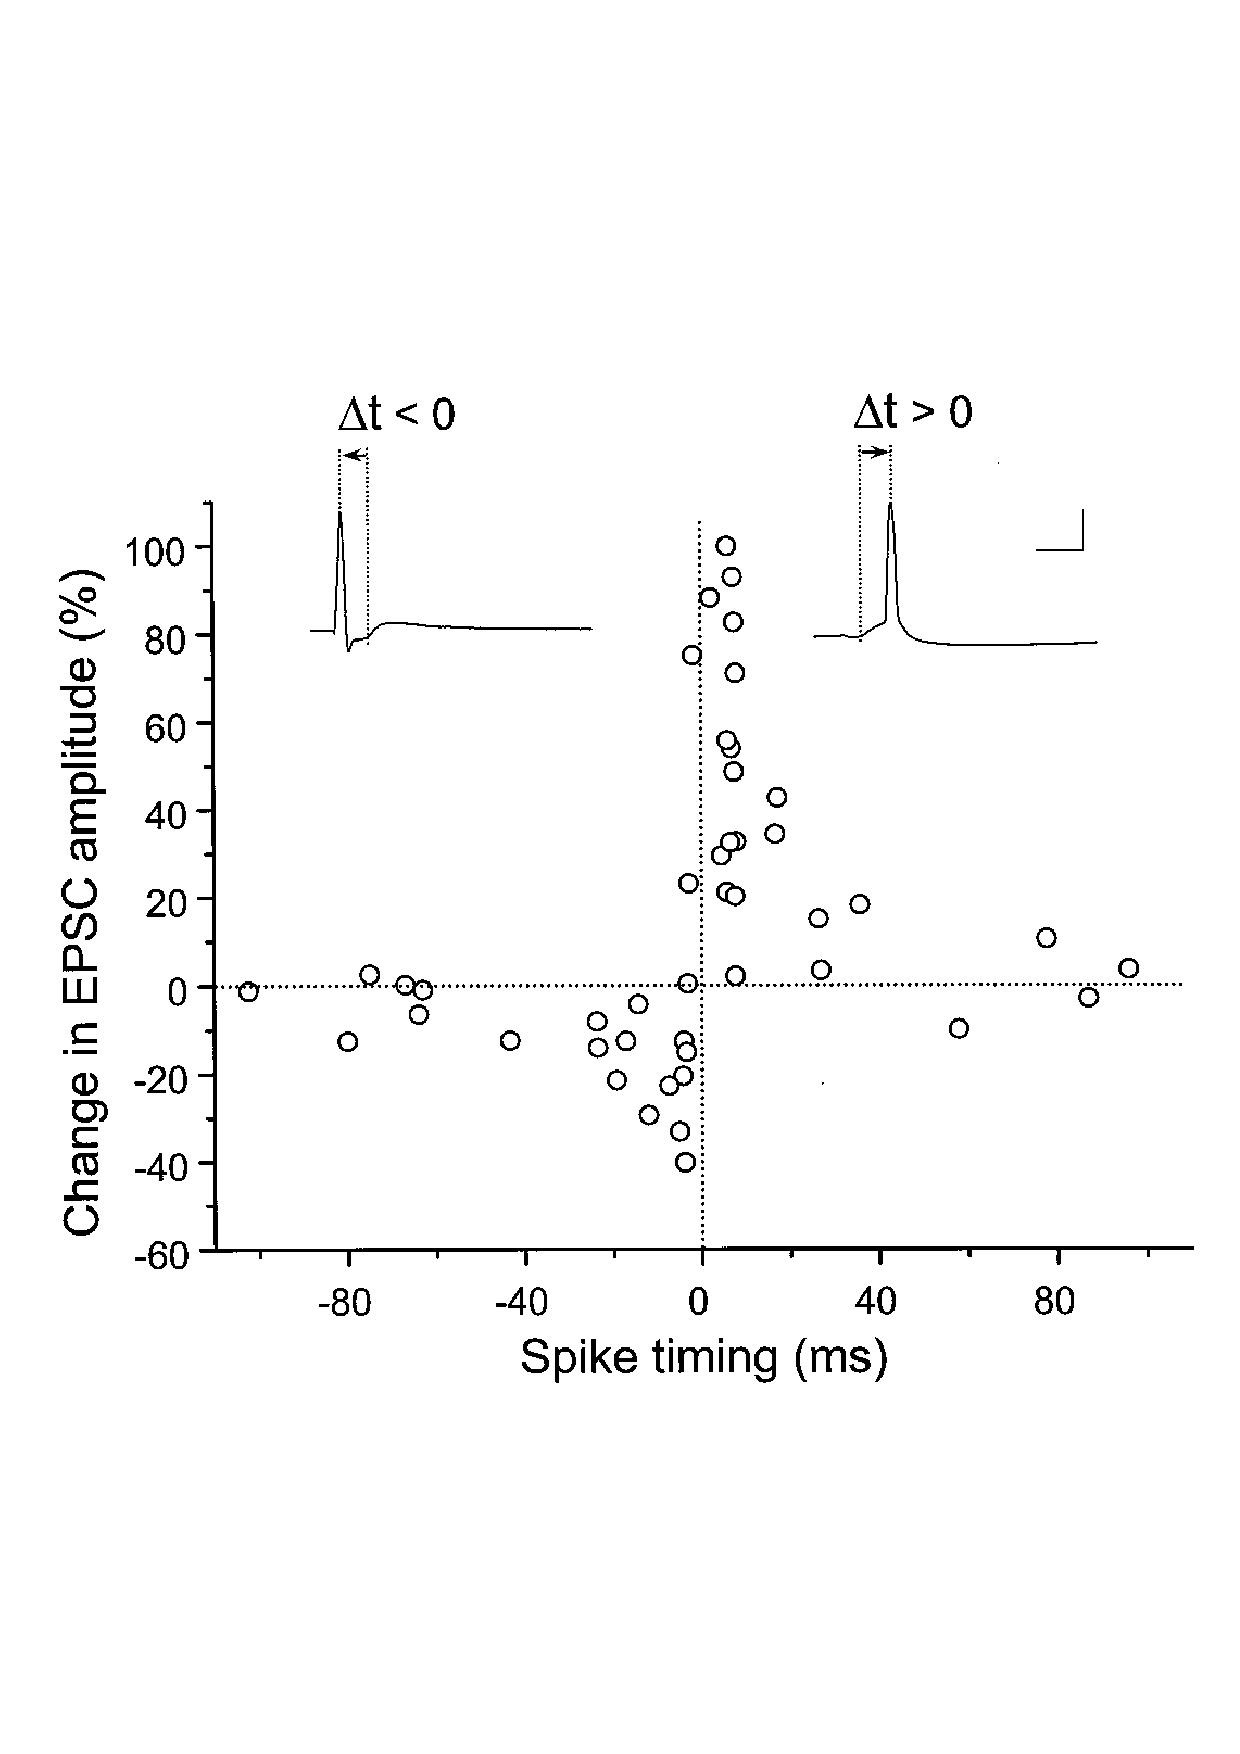
\includegraphics[width=\textwidth]{./figures/bi_stdp}
\vspace*{3mm}
\tiny{Bi \&  Poo (1998)\\
\textit{J Neurosci} \textbf{18}:10464--10472}
\column{0.6\textwidth}
\begin{itemize}
  \item LTP if presynaptic spike precedes postsynaptic spike by 10 ms
  \item LTD if order of spikes reversed
  \item repetitions of 60 pairs of spikes (single pair has no effect)
\end{itemize}

\end{columns}

\vspace*{3mm}

\small
{
\begin{itemize}
\item depends on exact timing of pre- and postsynaptic spikes on time scale of milliseconds
\item so called spike-timing dependent plasticity (STDP)
\end{itemize}
}

\end{frame}

\subsection{Spike-timing dependent plasticity}

\begin{frame}
  \frametitle{Spike-timing dependent plasticity (STDP)}

\includegraphics[width=0.5\textwidth]{./figures/stdp_exp}
\vspace*{3mm}
\tiny{Sjostrom et al. (2001)
\textit{Neuron.} \textbf{32}(6):1149--64}

\small
{
\begin{itemize}
\item synaptic strength (e.g. EPSP amplitudes) in data collected across several pairs of neurons reported to be unimodal
\end{itemize}
}

\end{frame}


\begin{frame}
  \frametitle{Spike-timing dependent plasticity (STDP)}

\includegraphics[width=0.9\textwidth]{./figures/stdp_exp1}
\begin{columns}
\column{0.4\textwidth}
\hspace*{1.5mm}
\includegraphics[width=0.8\textwidth]{./figures/stdp_exp2}
\vspace*{1mm}
\hspace*{3mm}\tiny{Sjostrom et al. (2001)\\
\hspace*{3mm}\textit{Neuron.} \textbf{32}(6):1149--64}
\column{0.6\textwidth}
\begin{itemize}
  \item 60 pre-post pairings at 0.1 Hz have no effect (C)
  \item same number of pairs at 40 Hz gives strong potentiation (B)
\end{itemize}

\end{columns}

\begin{itemize}
  \item depends on repetition frequency of pre-post spike-pairings
\end{itemize}

\end{frame}


\subsection{Homeostasis}

\begin{frame}
  \frametitle{Homeostasis of synaptic efficacies}

\begin{columns}
\column{0.35\textwidth}
\includegraphics[width=0.9\textwidth]{./figures/homeo}
\vspace*{3mm}
\tiny{Turrigiano et al. (1998)\\
\textit{Nature.} \textbf{391}:892--896}

\column{0.65\textwidth}
\small
{
\begin{itemize}
  \item chronic blockade of cortical culture activity increases amplitude of mEPSCs without changing their kinetics
\end{itemize}
}

\end{columns}

\vspace*{3mm}

\small
{
\begin{itemize}
  \item on a time scale of hours, rescaling of synaptic response amplitudes may occur
  \item useful to stabilize neuronal firing rates
\end{itemize}
}

\end{frame}

%%%%%%%%%%%%%%%%%%%%%%%%%%%%%%%%%%%%%%%%%%%%%%%%%%%%%%%%%%%%%%%%%%%%%%%%%%%%%%%

\section{Phenomenological models of synaptic plasticity}
%\subsection{Short-term plasticity (very briefly)}

%\begin{frame}
%  \frametitle{Phenomenological models of short-term plasticity}
%\includegraphics[width=0.85\textwidth]{./figures/std}\\
%\vspace*{3mm}
%\tiny{
%Left: experimental results adapted from Markram et al. (1998) \\
%Right: simulation results using Markram-Tsodyks model}
%\small{
%\begin{itemize}
%\item fast synaptic dynamics firmly established in biological literature (Markram et al. 1998; Gupta et al. 2000)
%\item well-accepted models exist (Abbott et al. 1997; Tsodyks et al. 1998)
%\end{itemize}
%}
%\end{frame}


\subsection{Spike-timing dependent plasticity}

\begin{frame}
  \frametitle{Phenomenological models of \\spike-timing dependent plasticity}
What do we need to specify a pair-based model of STDP?
  \begin{columns}[T]
\column{0.5\textwidth}
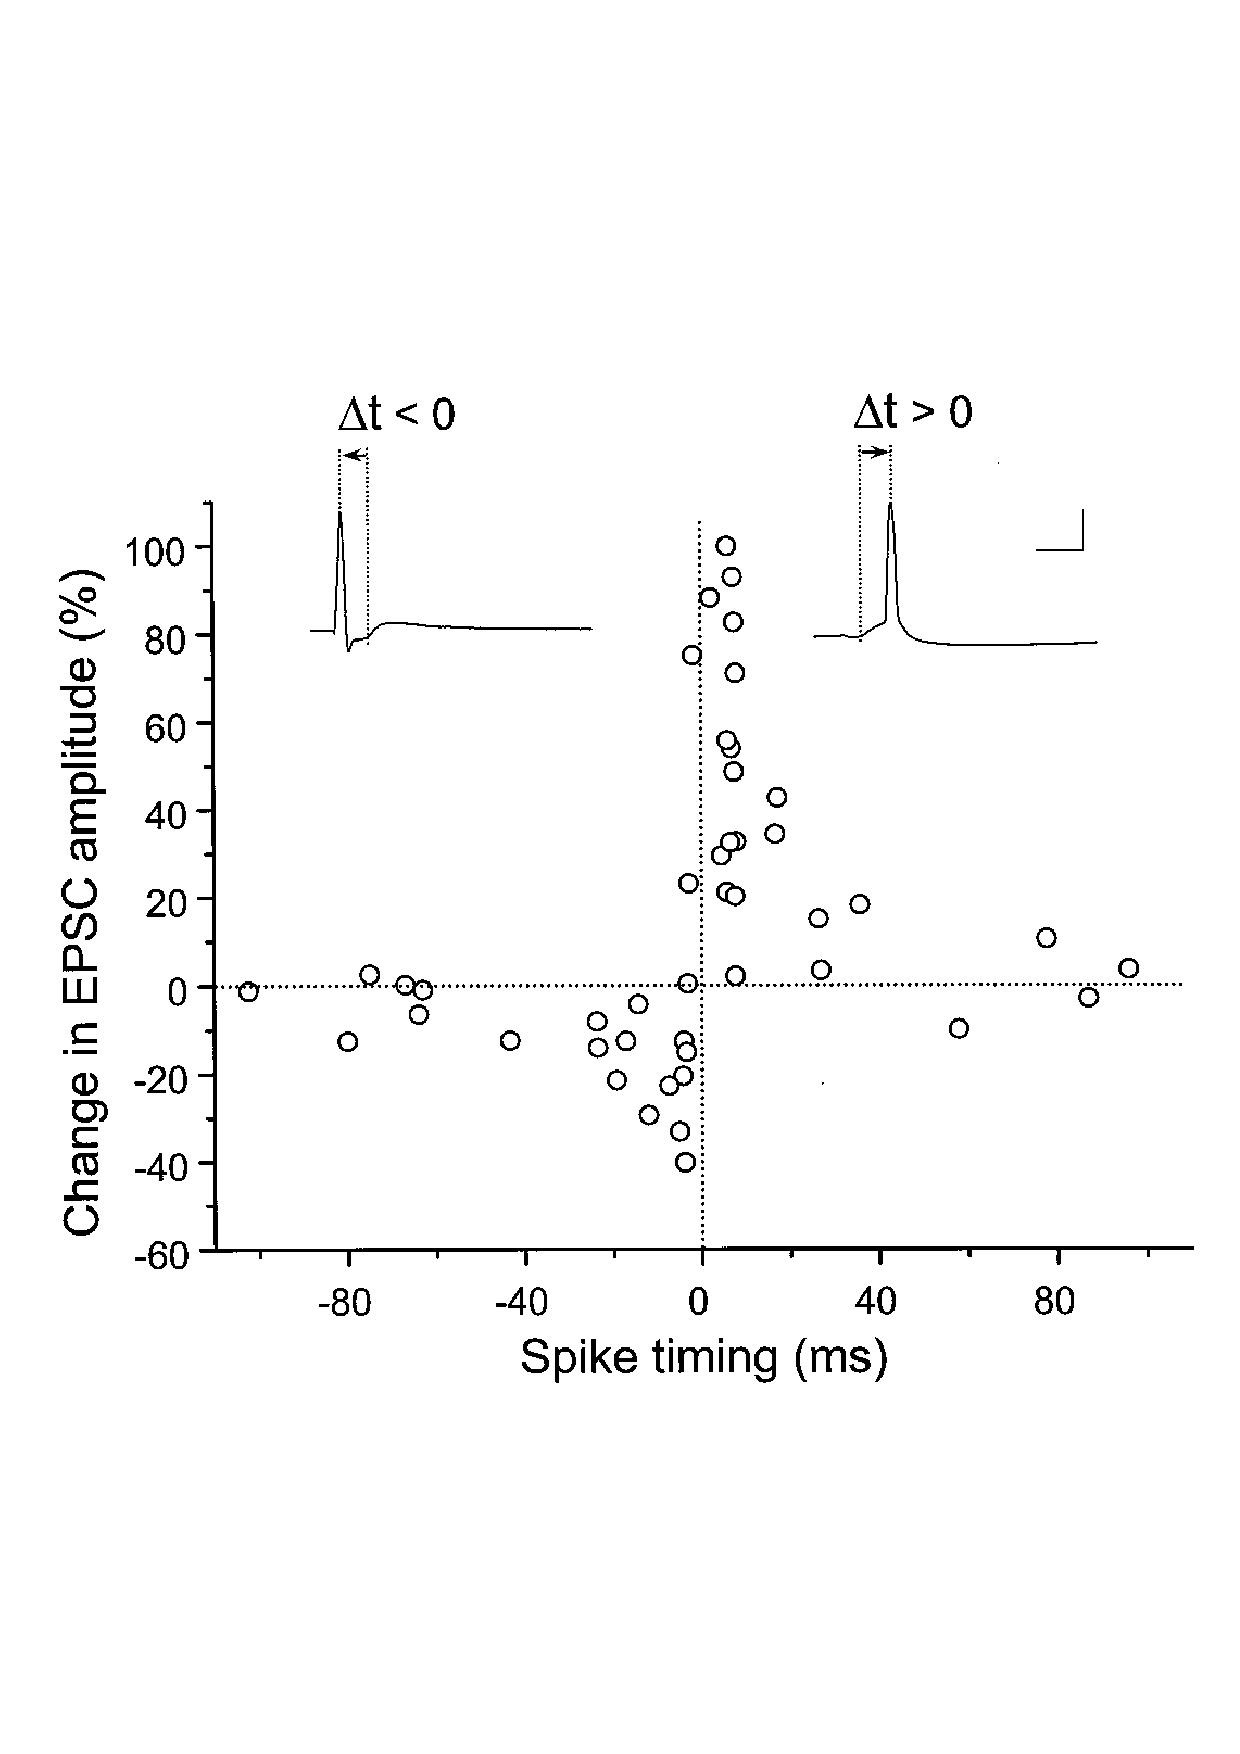
\includegraphics[width=\textwidth]{./figures/bi_stdp}
\vspace*{3mm}
\tiny{Bi \&  Poo (1998)\\
\textit{J Neurosci} \textbf{18}:10464--10472
}
\column{0.5\textwidth}
{\scriptsize
\begin{eqnarray*}
  \Delta w_{-} & = & -F_{-}\left(w\right)\mathrm{exp}\left(-\left|\Delta t\right|/\tau_{-}\right)\nonumber\\
 \Delta w_{+} & = & -F_{+}\left(w\right)\mathrm{exp}\left(-\left|\Delta t\right|/\tau_{+}\right)\nonumber
\end{eqnarray*}
}
\vspace*{-4mm}
\begin{itemize}
\setlength{\itemsep}{1.5mm}
\item weight dependence i.e. $F_{\pm}\left(w\right)$
\item spike pairing scheme
\item decomposition of synaptic delay into axonal and dendritic components
\item asymmetry of STDP kernel ($\alpha = \frac{F_{-}}{F_{+}}$)
\end{itemize}
\end{columns}
\vspace*{0.5mm}
{%\centering
\alert{all of these aspects are important\\ and should not be chosen arbitrarily}\\
}
\end{frame}


\begin{frame}
  \frametitle{Models of STDP: Weight Dependence}
\begin{center}
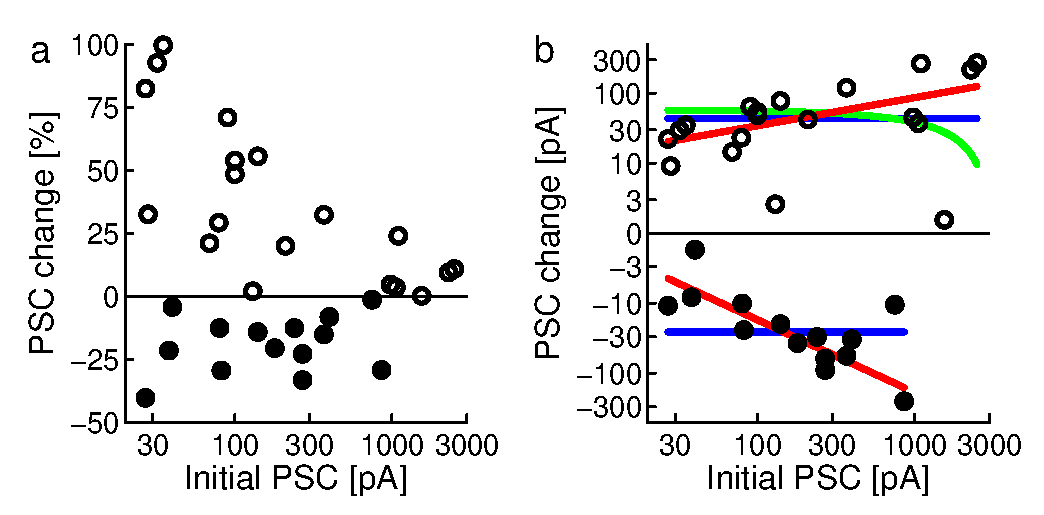
\includegraphics[width=0.85\textwidth]{./figures/weight_dep}
\end{center}
\small{
\begin{itemize}
\item Reanalysis of Bi \& Poo (1998) data shows that the commonly used \textcolor{blue}{additive} model ($F_{-}=A_{-}$,$F_{+}=A_{+}$) is not a good fit for the data.
\item Depression data are best fit by a \textcolor{green}{multiplicative}/\textcolor{red}{power law} model   ($F_{-}=A_{-}w^{-1}$ ) 
\item Potentiation data are best fit by a \textcolor{red}{power law} model\\ ($F_{+}=A_{+}w^{\mu}$, $\mu=0.4$)
\end{itemize}
}
\end{frame}


\begin{frame}
  \frametitle{Models of STDP:\\Distribution of synaptic weights}
  \begin{columns}
    \column{0.4\textwidth}

    \vspace*{5mm}
    \includegraphics[width=\textwidth]{./figures/fix_point}
    \column{0.6\textwidth}
    \includegraphics[width=\textwidth]{./figures/add_mul_dists}
    \hspace*{-5cm}
    \raisebox{4.3cm}[0cm][0cm]{%
        \scriptsize{additive \hspace*{13mm} multiplicative}
    }
  \end{columns}
\begin{itemize}
  \item all weight dependent models exhibit a stable fixed point and generate a unimodal distribution (\textcolor{green}{multiplicative}, \textcolor{red}{power law}, \textcolor{magenta}{G{\"u}tig}, \textcolor{cyan}{Van Rossum})
  \item the \textcolor{blue}{additive} model does not have a stable fixed point and produces a bimodal distribution
\end{itemize}
\end{frame}


\begin{frame}
\frametitle{Models of STDP: Spike Pairing Scheme}
\begin{columns}[T]
  \column{0.32\textwidth}
    all-to-all...

    \includegraphics[width=\textwidth]{./figures/izhik_a2a}
    \column{0.305\textwidth}
    ... or nearest neighbour?

    \vspace*{-3.5mm}
    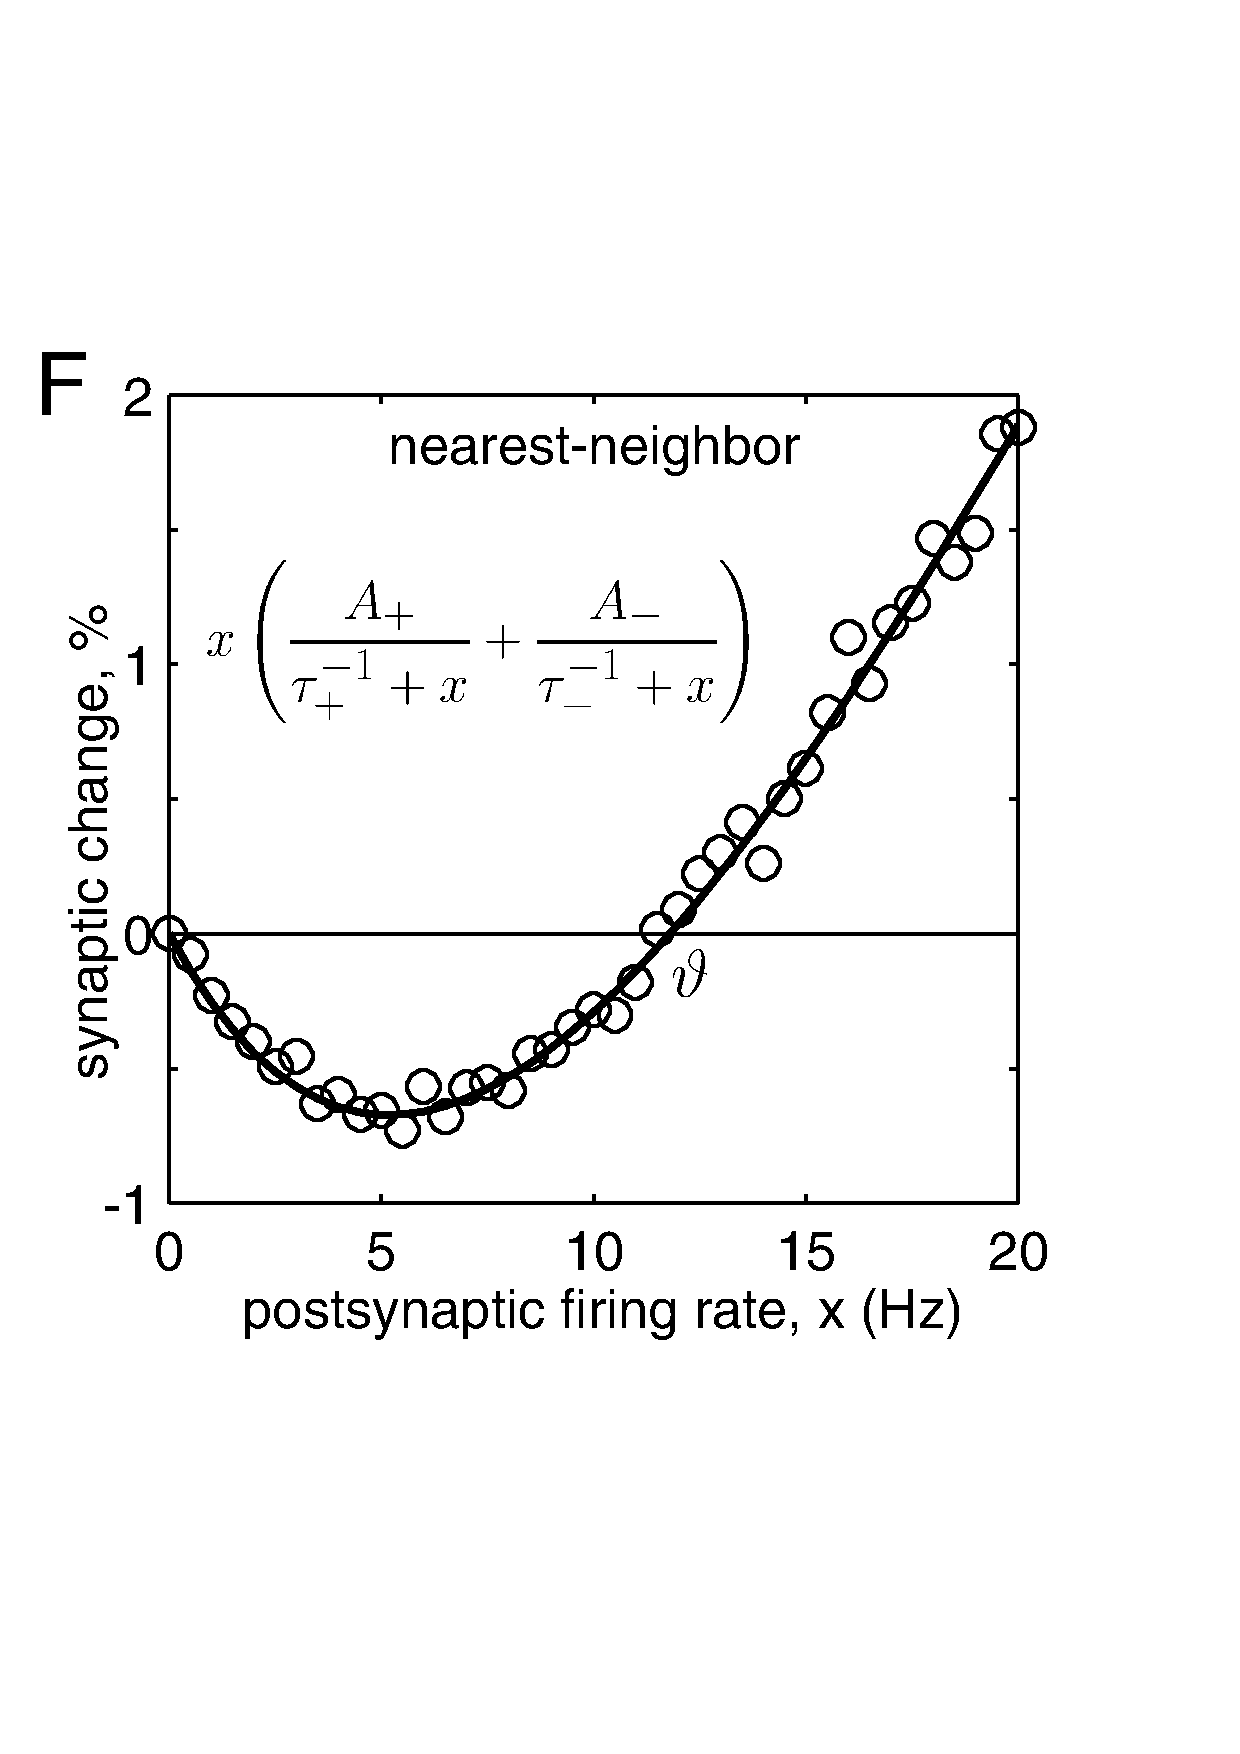
\includegraphics[width=\textwidth]{./figures/izhik_nn}
    \column{0.375\textwidth}

    \hspace*{3mm}...but which nearest\\\hspace*{5mm} neighbour?
    \includegraphics[width=\textwidth]{./figures/spike_pairing}
\end{columns}
\raisebox{0.5cm}[0cm][0cm]{% 
        \tiny{Izhikevich \& Desai (2003) \textit{Neural Comput} \textbf{15}:1511--1523}
    }
\begin{itemize}
\item there are many possible spike pairing schemes
\item they can give qualitatively different results {\scriptsize{(e.g. Kempter et al. 2001; Morrison et al. 2007)}}
\item see Burkitt et al (2004) for copious analysis
\end{itemize}
\end{frame}


\begin{frame}
  \frametitle{Models of STDP: Synaptic Delays}
  \begin{center}
    \includegraphics[width=\textwidth]{./figures/synaptic_delays}
  \end{center}
\begin{itemize}
  \item The synaptic drift depends on the \textcolor{red}{cross-correlation with respect to the synapse}
  \item This is shifted from to the left or right of the (measurable) \textcolor{dgray}{cross-correlation with respect to the soma} depending on whether the synaptic delay is largely axonal (a) or dendritic (c)
  \item Therefore the same STDP rule coupled with the same network dynamics can give rise to either net depression, no change, or net potentiation
\end{itemize}
\end{frame}


\begin{frame}
\frametitle{Models of STDP: Beyond Pair Effects}
Many features of STDP cannot be explained by pair-based rules:
\begin{columns}[T]
    \column{0.5\textwidth}
    %\vspace*{5mm}
\begin{center}
    Frequency dependence
\end{center}
    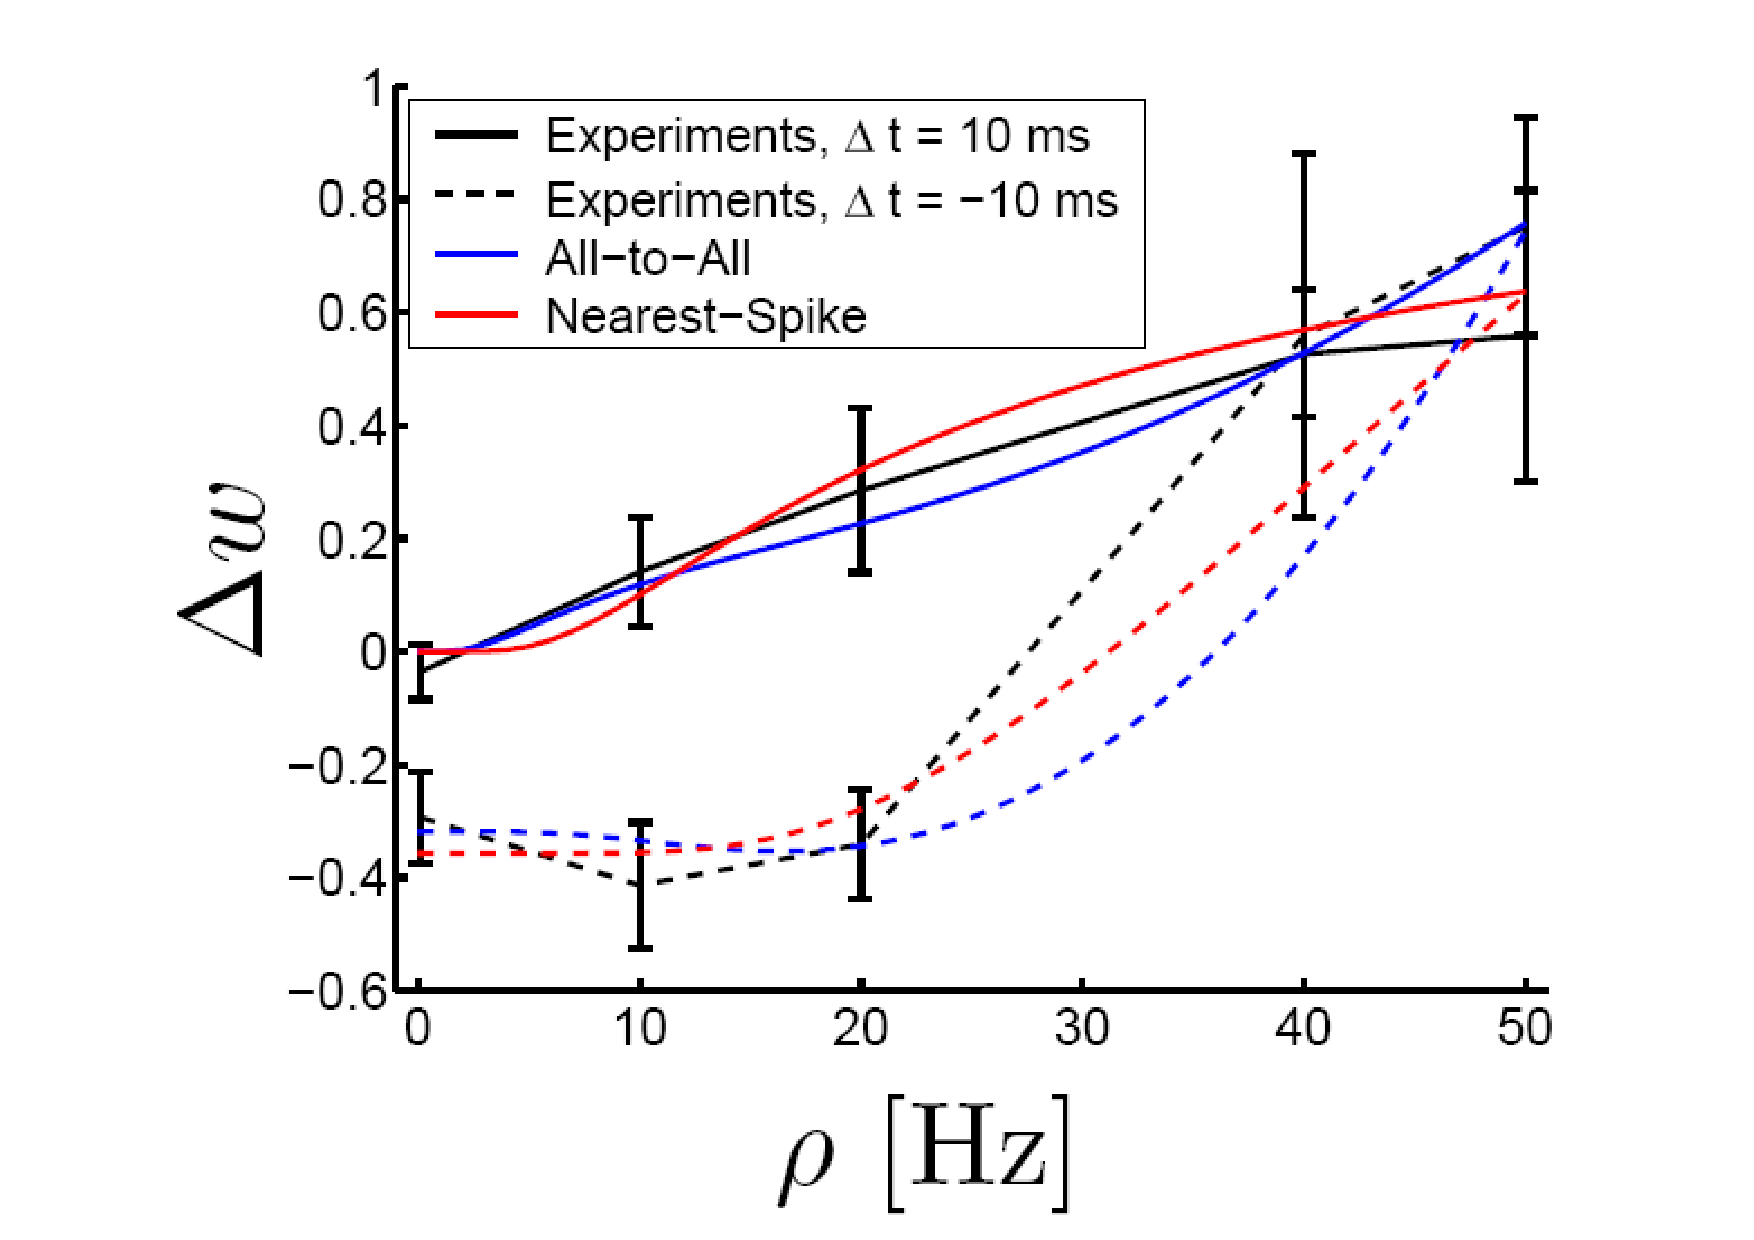
\includegraphics[width=\textwidth]{./figures/triplet-frequency}

    \tiny{Data: Sjostrom et al. (2001) \textit{Neuron} \textbf{32}:1149--1164}\\
    \tiny{Modelling: Pfister et al. (2006) \textit{J Neurosci} \textbf{26}:9673--9682}
    \tiny{Modelling: Also see Clopath et. al (2010) \textit{Front.Synap Neurosci.}, Shouval et. al (2010) \textit{Front. Comp. Neurosci.}, Costa et al. (2015) \textit{eLife} }
    \column{0.5\textwidth}
\begin{center}Burst dependence\end{center}
    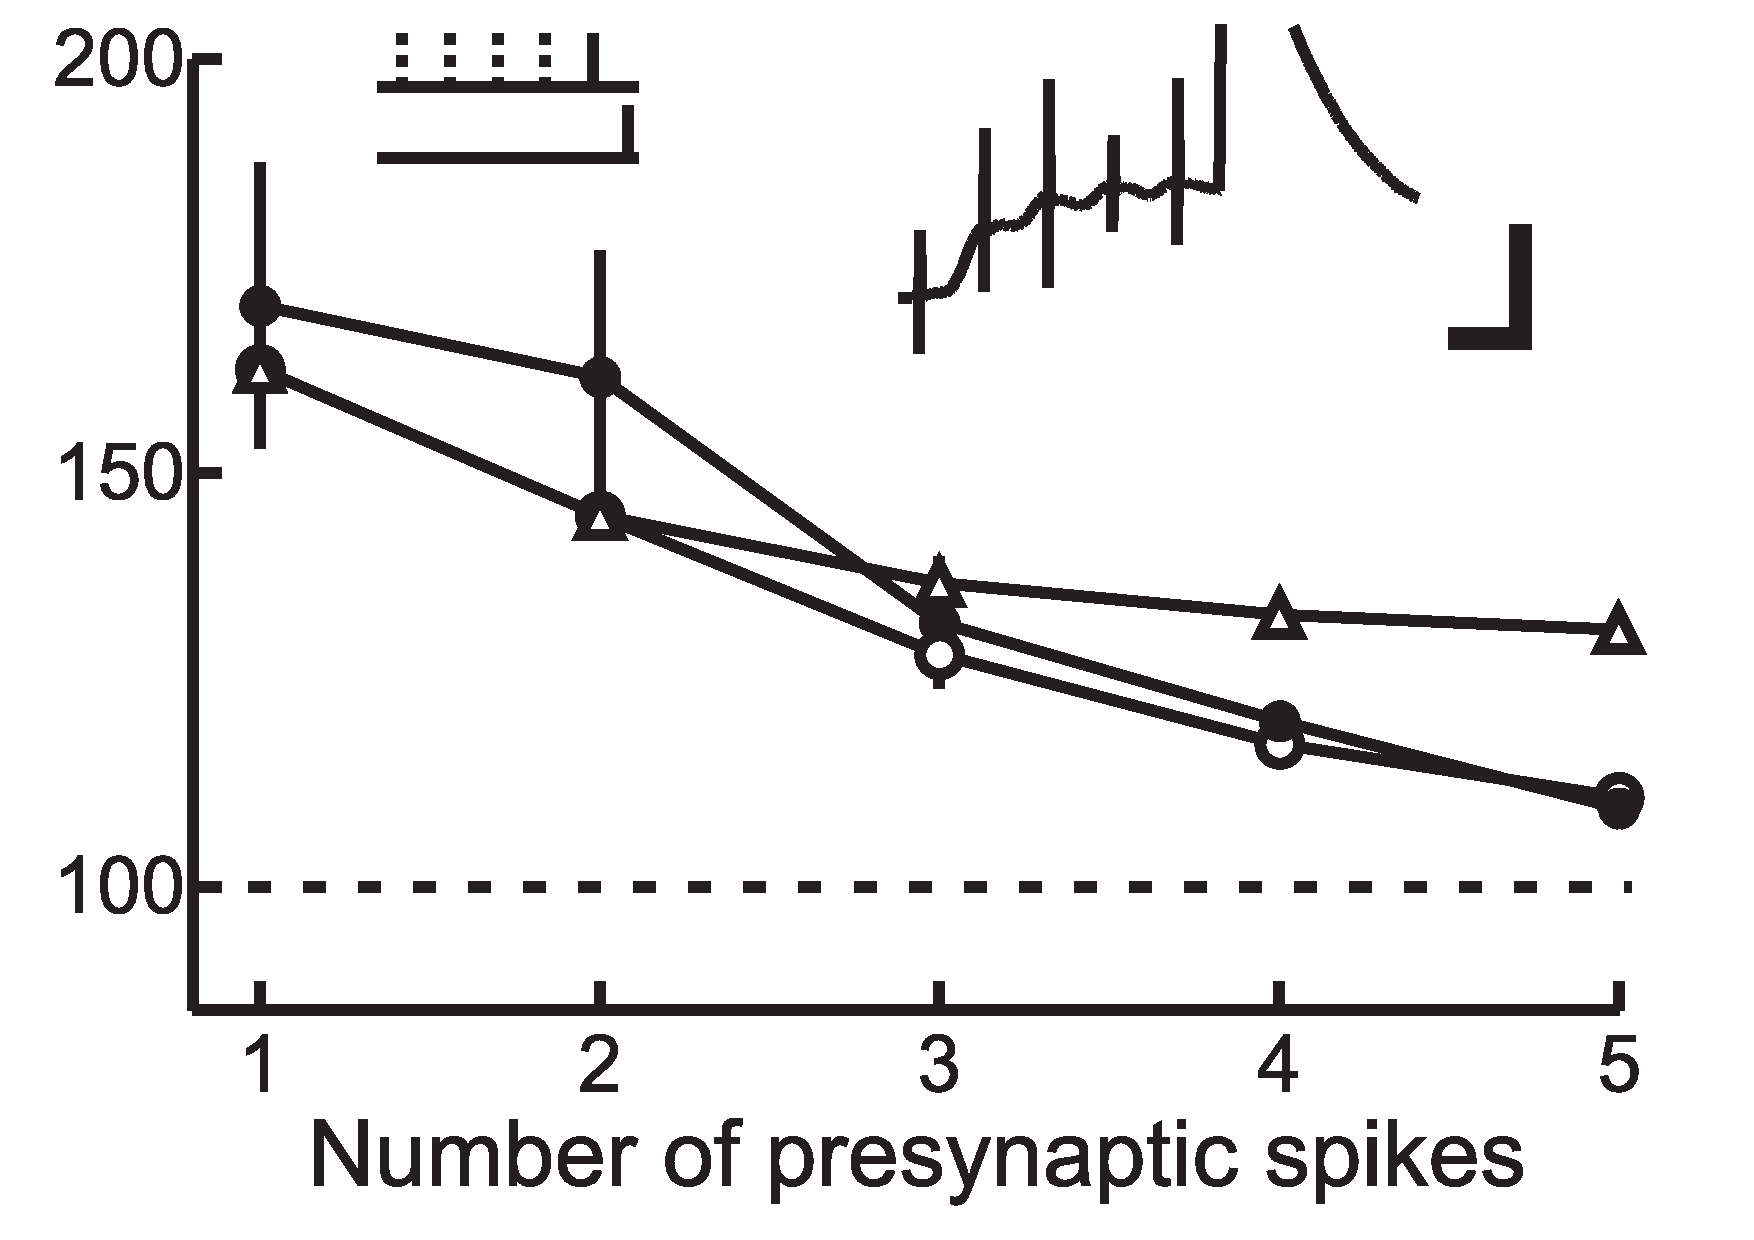
\includegraphics[width=\textwidth]{./figures/froemke_burst}  

    \tiny{Data and modelling: Froemke et al. (2006) \textit{J Neurophysiol} \textbf{95}:1620--1629}
  \end{columns}
\hspace*{5.5cm}\raisebox{1.3cm}[0cm][0cm]{\rotatebox{90}{\scriptsize{\% Change EPSP Slope}}}

\vspace*{3mm}
\alert{There is generally no cross-compatibility between models accounting for these features}
\end{frame}
%%%%%%%%%%%%%%%%%%%%%%%%%%%%%%%%%%%%%%%%%%%%%%%%%%%%%%%%%%%%%%%%%%%%%%%%%%%%%%%


\section{Beyond spike-pairings}
\subsection{Influence of neuromodulators}


\begin{frame}
\frametitle{Is pre- and post-spike timings enough to model learning?}

\begin{columns}[T]
    \column{0.5\textwidth}
    

    \begin{itemize}
            \item Neuromodulators are neurotransmitter which are thought influence more that just one synapse but diffuse in larger cortical areas
            \item Therefore considered to be non-locally modulating synaptic transmission
            \item I.e. Dopamine, Serotonine, Acetylcholine, ...
    \end{itemize}

    \column{0.5\textwidth}
    \begin{center}
        Dopaminergic pathway
    \end{center}
    \includegraphics[width=\textwidth]{./figures/dopa_path.png}

  \end{columns}


\end{frame}

\begin{frame}
\frametitle{Effects of Neuromodulators on STDP}

    \begin{columns}[T]
    \column{0.3\textwidth}
    

    \begin{itemize}
            \item Dopamine permits induction of LTP and LTD in striatal neuron 
            \item If dopamine is blocked, no plasticity is induced
    \end{itemize}

    \column{0.7\textwidth}
    \includegraphics[width=\textwidth]{./figures/dopa_blocked}

    \tiny{Pawlak and Kerr, 2008 / 2010}

  \end{columns}


\end{frame}



\begin{frame}
\frametitle{Effects of Neuromodulators on STDP}
    \begin{columns}[T]
    \column{0.5\textwidth}
    

    \begin{itemize}
        \item Dopamine can switch the STDP window in hippocampus
        \item Less spikes are necessary to induce STDP under the influence of dopamine 
    \end{itemize}

    \column{0.5\textwidth}
    \includegraphics[width=0.8\textwidth]{./figures/dopa_switch}

    \tiny{Zhang et al., 2009, Pawlak and Kerr, 2010}

  \end{columns}

\end{frame}



\begin{frame}
\frametitle{Effects of neuromodulators on STDP}

    \includegraphics[width=\textwidth]{./figures/effect_table}

    \tiny{Pawlak and Kerr, 2010}

\end{frame}

\begin{frame}
\frametitle{Functional aspects of dopamine}
    \begin{columns}[T]
    \column{0.5\textwidth}
    

    \begin{itemize}
        \item Dopamine is probably the most studied neuromodulator
        \item Involved in conditioning as reward and punishment signal
        \item Credit assignment problem
        \item Theoretical prediction of 'eligibility traces'
    \end{itemize}

    \column{0.5\textwidth}
    \includegraphics[width=0.8\textwidth]{./figures/schultz_rpe}

    \tiny{Schultz et al. 1997}

  \end{columns}

\end{frame}


\begin{frame}
\frametitle{Effective timescales of dopamine}
    \begin{columns}[T]
    \column{0.4\textwidth}
    

    \begin{itemize}
        \item In different regions neuromodulators effect STDP with different timescales
        \item A) Striatum ($\sim 1\text{s}$) 
        \item B) Cortex ($\sim 5\text{s}$) 
        \item C) Hippocampus ($\sim \text{min}$) 
    \end{itemize}

    \column{0.6\textwidth}
    \includegraphics[width=1.0\textwidth]{./figures/dopa_timeconst}

    \tiny{Gerstner et al. 2018, Yagishita et al. 2014, He et al. 2015, Bittner et al. 2017 }

  \end{columns}

\end{frame}





\begin{frame}
\frametitle{Conclusions}
\begin{itemize}
\item A modeller needs to specify a complete model despite lack of clear experimental evidence
\item These choices can have profound consequences
\item Almost all network modelling papers fail to consider whether the effects shown are artifacts of their specific choices
\item There is so far no phenomenological model which accounts for all the nonlinearites exhibited by STDP 
\item For those who want to know more...
\end{itemize}
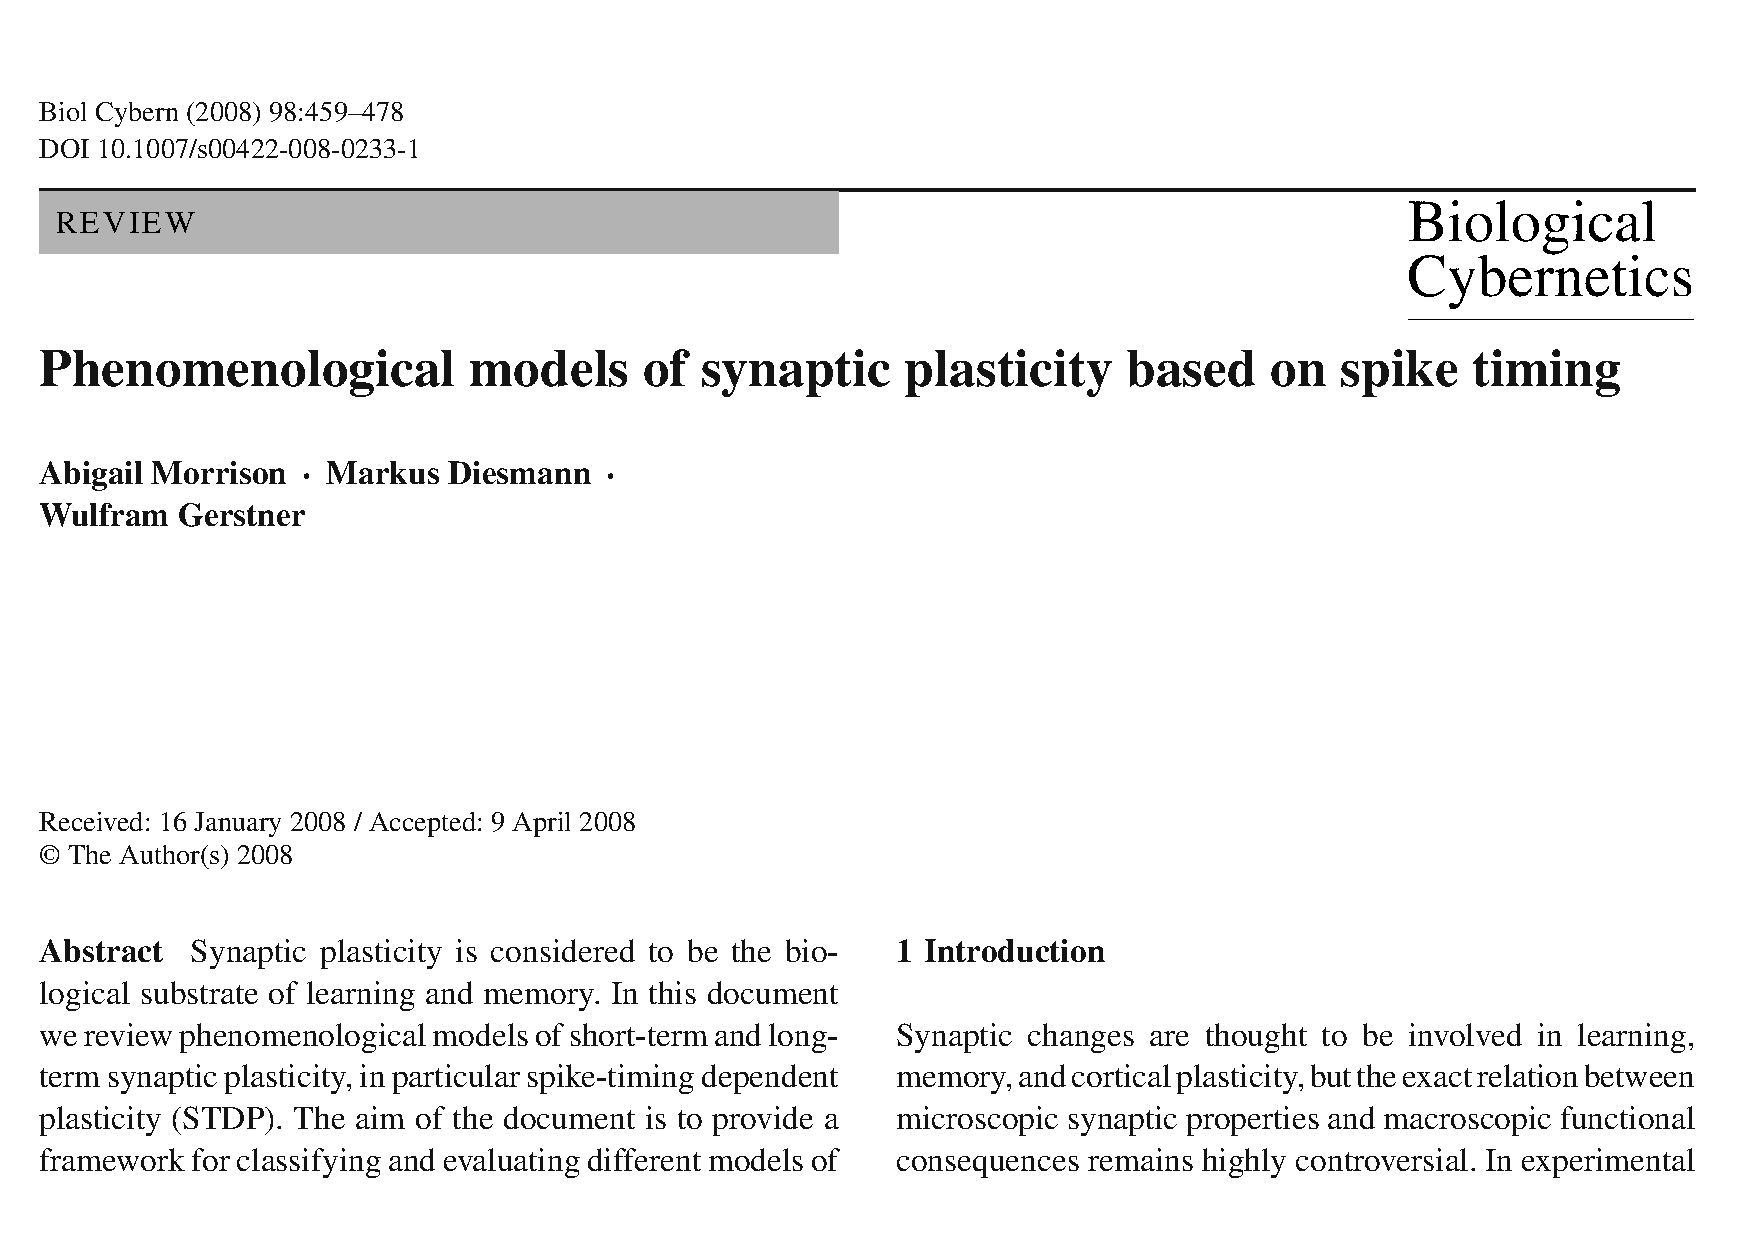
\includegraphics[width=\textwidth]{./figures/bio_cyb}
\end{frame}


\end{document}
